% !TEX program = xelatex
\documentclass[11pt,letterpaper]{article}
\usepackage[textwidth=6.55in,textheight=9.1in,top=.85in]{geometry}
\usepackage{pifont}
\usepackage{fontspec,newtxmath,amsmath,graphicx,booktabs,array,longtable,multirow}
\usepackage[numbers,square,sort&compress]{natbib}
\usepackage{xurl,hyperref,caption,fancyhdr,microtype,setspace,titlesec,textcomp}
\usepackage{placeins}
\usepackage{float}
\setmainfont{texgyretermes-regular.otf}[BoldFont=texgyretermes-bold.otf,ItalicFont=texgyretermes-italic.otf,BoldItalicFont=texgyretermes-bolditalic.otf]
\hypersetup{colorlinks=true,linkcolor=black,citecolor=black,urlcolor=black,pdftitle={From Tokenizer to PDE Discovery}}
\captionsetup{font=small,labelfont=bf,labelsep=quad,skip=5pt}
\setlength{\parindent}{1em}\setlength{\parskip}{2pt}\setstretch{1.05}
\setlength{\textfloatsep}{12pt}\setlength{\floatsep}{10pt}\setlength{\intextsep}{10pt}
\setlength{\emergencystretch}{1.5em}\setlength{\tabcolsep}{4pt}\renewcommand{\arraystretch}{1.15}
\titleformat{\section}{\large\bfseries}{\thesection}{1em}{}
\titleformat{\subsection}{\normalsize\bfseries}{\thesubsection}{1em}{}
\titlespacing*{\section}{0pt}{13pt}{6pt}
\titlespacing*{\subsection}{0pt}{9pt}{4pt}
\pagestyle{fancy}\fancyhf{}\fancyfoot[C]{\small\thepage}\setlength{\headheight}{13pt}\setlength{\headsep}{18.9pt}\addtolength{\topmargin}{6.1pt}\setlength{\footskip}{38pt}\renewcommand{\headrulewidth}{0pt}
\title{From Tokenizer to PDE Discovery}\author{}\date{}
\makeatletter\renewcommand{\maketitle}{\begin{center}{\LARGE\bfseries\@title\par}\end{center}\vspace{8pt}}\makeatother
\newcommand{\fig}[3]{\begin{figure}[!htbp]\centering\includegraphics[width=#2\linewidth]{figures/#1.pdf}\caption{#3}\label{fig:#1}\end{figure}}
\begin{document}
\maketitle\thispagestyle{fancy}
\section{Background}
\subsection{Preliminaries}
\paragraph{EqGPT.}
EqGPT collects PDEs from mathematical handbooks, encodes basic terms and operators into a generative representation of equations (GRE), and trains an autoregressive Transformer to predict the next token. In parallel, observational data are used to train a surrogate network for the field. This network reconstructs the observed field and computes derivatives by automatic differentiation, providing numerical data for evaluating candidate equations.

The discovery stage follows a generation--evaluation--fine-tuning loop. The model samples tokens from a start symbol until it produces a complete equation structure. The coefficients are then fitted by least squares using data from the surrogate network, and each equation is scored using its goodness of fit and number of terms. The ten highest-scoring candidates are used for supervised fine-tuning (SFT), and the updated model generates candidates for the next round. After the loop, the highest-scoring structure is selected, and its coefficients are further optimized.

\begin{figure}[H]
\centering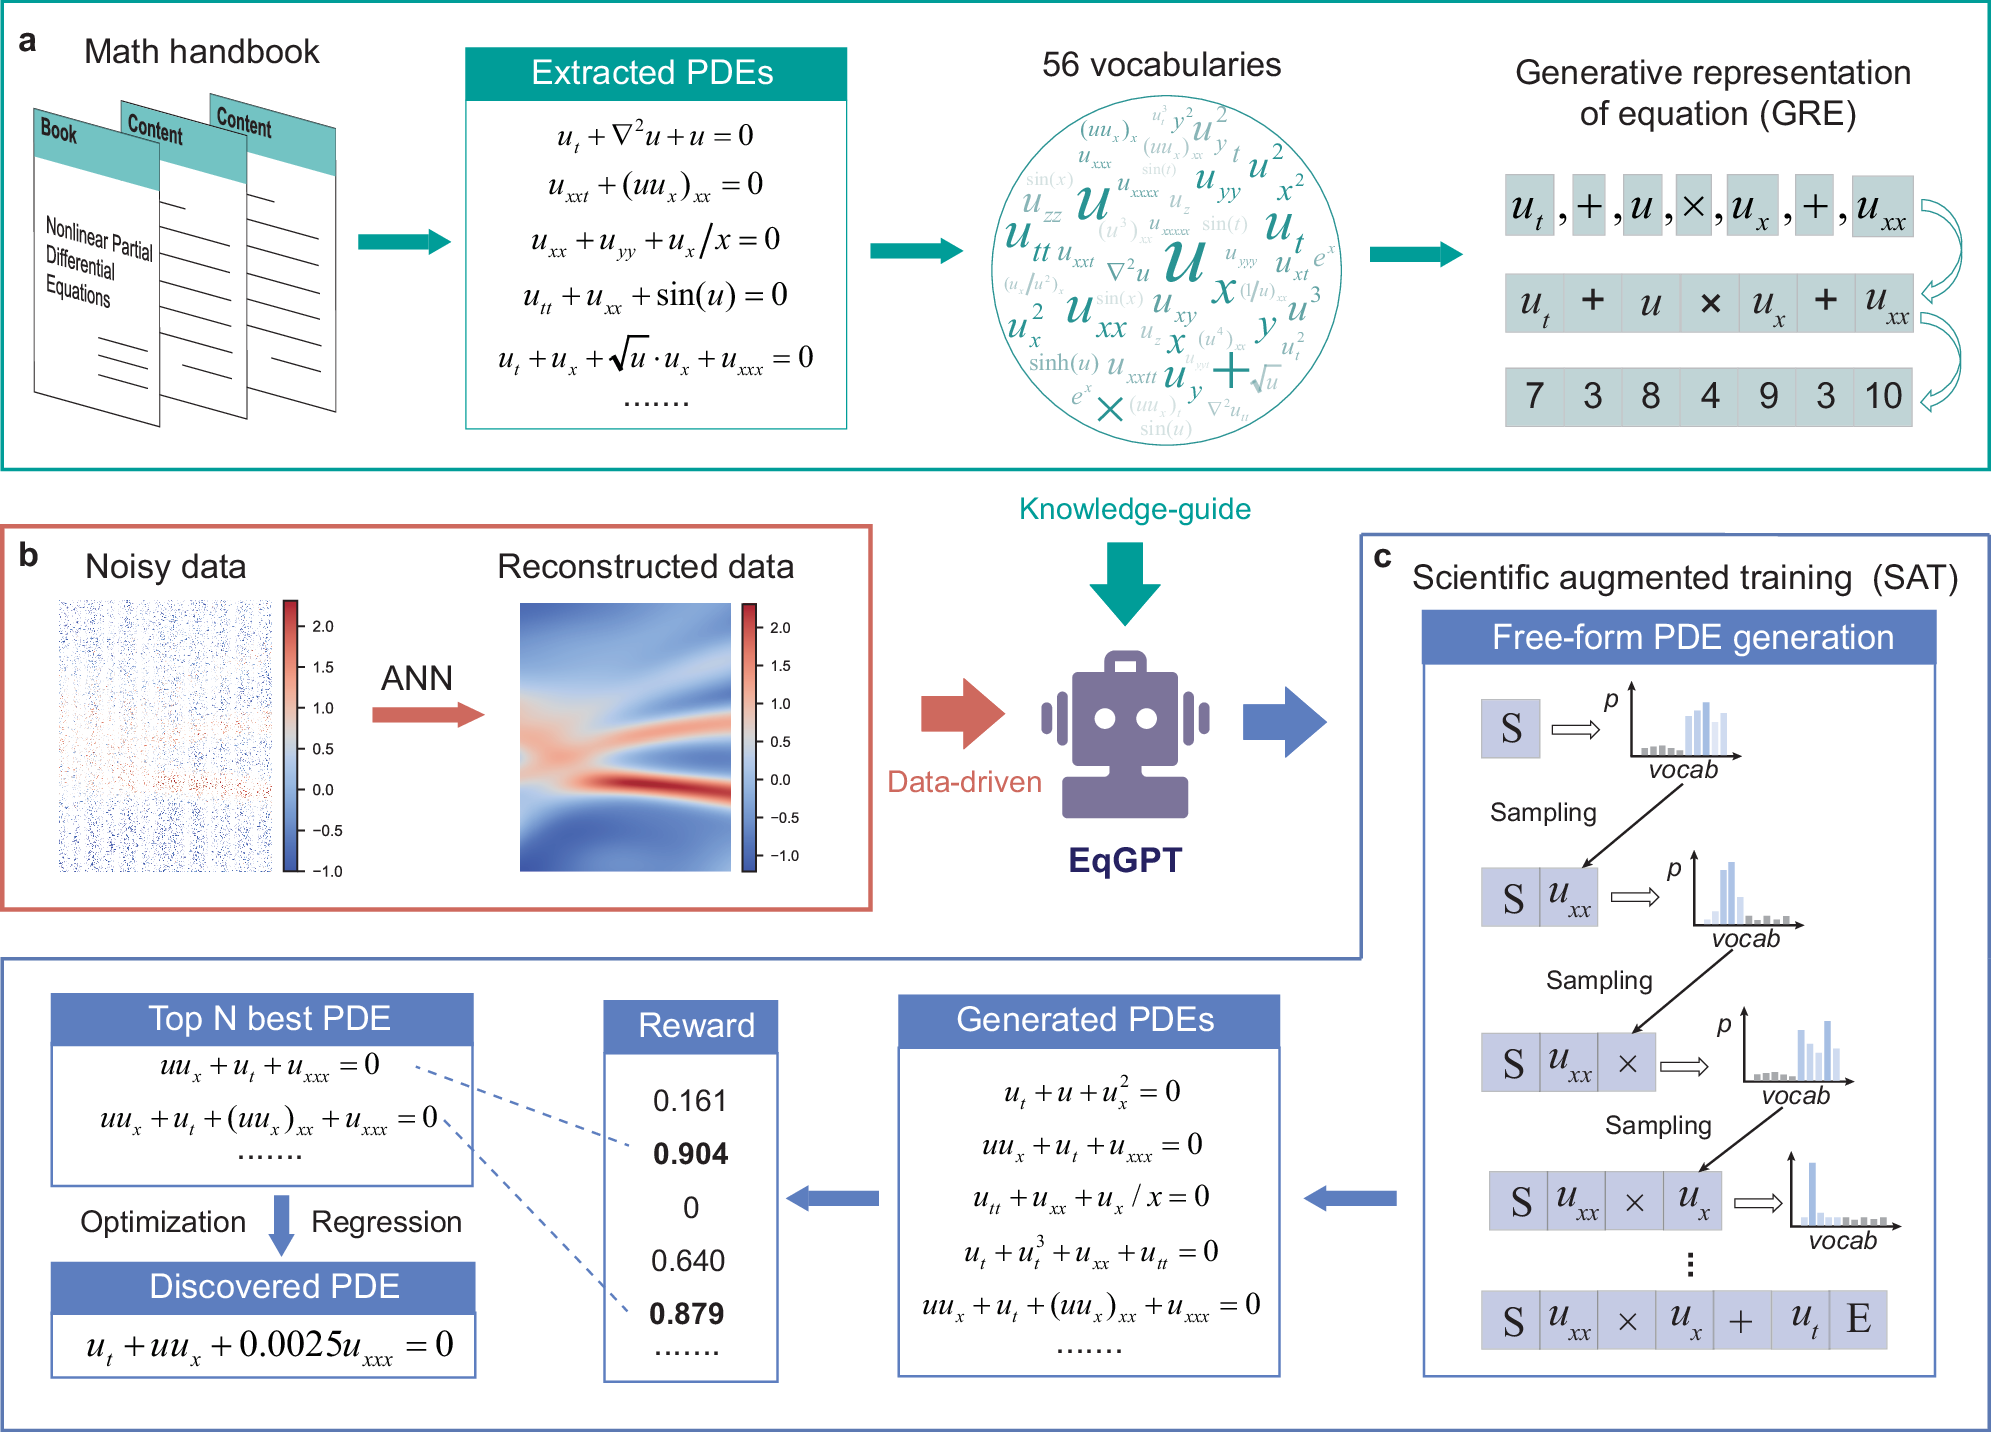
\includegraphics[width=\linewidth]{figures/eqgpt_original.png}
\caption*{\textbf{Workflow diagram from the original EqGPT paper.}}
\end{figure}

\subsection{Differences from EqGPT}\label{subsec:changes}
We make two changes to the EqGPT framework.

\textbf{Replace the tokenizer.} Original EqGPT directly encodes GRE basic terms and operators; we use AST-BPE as the tokenizer. The vocabulary is trained on the unaugmented corpus, while the Transformer is trained on the augmented corpus.

\begin{samepage}
\textbf{Remove SAT grammar constraints during generation.} The AST-BPE model directly generates LaTeX according to token probabilities, without using SAT in EqGPT (which uses human-defined rules to ensure valid PDE outputs).
\end{samepage}

\section{Experimental Setup}
\subsection{Eight PDE Cases}
We use the eight single-field PDE cases in Table~\ref{tab:cases} to examine whether the model can discover the corresponding target equation from data.

\begin{table}[!htbp]
\caption{Eight target equations. $u=u(x,t)$, and subscripts denote partial derivatives. PDE-divide is evaluated in the region $x\ne0$.}\label{tab:cases}
\centering\small
\begin{tabular*}{\linewidth}{@{\extracolsep{\fill}}ll@{}}\toprule
Case & Target equation\\\midrule
Wave & $u_{tt}-u_{xx}=0$\\
Convection--diffusion & $u_t+u_x-0.25u_{xx}=0$\\
Klein--Gordon & $u_{tt}-0.5u_{xx}+5u=0$\\
Burgers & $u_t+uu_x-0.1u_{xx}=0$\\
Eq.\ 6.2.12 & $u_t+0.1u_{xt}+0.1u_x=0$\\
PDE-divide & $u_t+u_x/x+0.25u_{xx}=0$\\
KdV & $u_t+uu_x+0.0025u_{xxx}=0$\\
Chaffee--Infante & $u_t-u_{xx}+u-u^3=0$\\\bottomrule
\end{tabular*}
\end{table}

\subsection{Training Corpora and Splits}
The small and large corpora contain 212 and 636 equations, respectively. The large corpus adds 424 equations to the small corpus, covering transport, reaction--diffusion, wave, elliptic, dispersive, and higher-order PDEs.

The upstream and downstream tasks use the same large corpus, with the actual splits shown in Table~\ref{tab:splits}.
\begin{table}[H]
\caption{Corpus splits for the upstream and downstream tasks. Downstream testing uses the eight PDE cases in Table~\ref{tab:cases}; no separate corpus test set is used.}\label{tab:splits}
\centering\small
\begin{tabular*}{\linewidth}{@{\extracolsep{\fill}}llrrrr@{}}\toprule
Task & Corpus & Total & Training & Validation & Test\\\midrule
Upstream tokenization & Large & 636 & 509 & 64 & 63\\
Downstream discovery & Small & 212 & 191 & 21 & --\\
Downstream discovery & Large & 636 & 572 & 64 & --\\\bottomrule
\end{tabular*}
\end{table}

\subsection{Training and Search Parameters}
All models use a six-layer Transformer. Pretraining uses cosine annealing and validation-based early stopping, with a maximum of 200 epochs. Each PDE discovery run has five search rounds. Each round obtains 400 successfully scored candidates, followed by five SFT epochs using high-scoring candidates. In the main experiments, all models use 80\% model-based sampling and 20\% random sampling, following the original EqGPT configuration. Random sampling has a substantial effect on discovery results; the comparisons are presented in Appendix~\ref{app:sampling}.

Experiments use three seeds: 525, 526, and 527.\footnote{All experimental results in the main text use seed 525.} Full parameters and results for the other seeds are provided in Appendices~\ref{app:params} and~\ref{app:seeds}.

\subsection{Evaluation Metrics}
\paragraph{Tokenization performance.}
\begin{itemize}\setlength{\itemsep}{2pt}\setlength{\parsep}{0pt}
\item \textbf{Compression ratio.} $C=N_{\rm initial}/N_{\rm final}$ is the number of tokens obtained with the initial vocabulary divided by the number obtained with the final vocabulary.
\item \textbf{Command integrity.} $I_{\rm cmd}$ is the proportion of complete LaTeX commands that are not split internally.
\item \textbf{Number integrity.} $I_{\rm num}$ is the proportion of complete numeric strings that are not split internally.
\item \textbf{Vocabulary utilization.} Newly added tokens are tokens learned through BPE merges, excluding initial characters and control symbols. It is defined as
\begin{equation}
 U=\frac{\text{number of distinct newly added tokens used}}{\text{total number of newly added tokens}}.
\end{equation}
For example, suppose a vocabulary adds five token types: \verb|u_t|, \verb|u_x|, \verb|u_{xx}|, \verb|\sin|, and \verb|\cos|. If the final encoding of the validation set uses only the first two, then $U=2/5=40\%$. Each token type is counted once, regardless of how often it occurs. This metric measures how broadly the newly added tokens are used in the evaluation data.

\end{itemize}

\paragraph{PDE discovery.}
Two equations have the same structure if their structures are identical when coefficients are ignored.
\begin{itemize}\setlength{\itemsep}{2pt}\setlength{\parsep}{0pt}
\item \textbf{Top1.} Whether the candidate equation with the highest final reward has the same structure as the target equation.
\item \textbf{Top10.} Whether any of the ten candidate equations with the highest final rewards has the same structure as the target equation.
\item \textbf{Reward.} Numerical scoring follows EqGPT:
\begin{equation}\label{eq:reward}
 r=\left(1-0.2\log_{10}M\right)R^2.
\end{equation}
\end{itemize}

\section{Experiments and Results}
\subsection{Upstream Tasks}
We conduct three upstream experiments to study tokenizer performance, the effect of vocabulary size on AST-BPE, and tokenizer generalization.

First, we evaluate the tokenizers on the 636-equation corpus (Table~\ref{tab:upstream}). We split the data as shown in Table~\ref{tab:splits}, learn the AST-BPE vocabulary using only the training set, and apply AST-BPE, Qwen2.5, Llama 3, and \texttt{o200k\_base} to the same test set to compute tokenization metrics. At vocabulary sizes of 300 and 450, AST-BPE preserves complete LaTeX commands and achieves compression ratios of 6.983 and 8.497, respectively, compared with 1.725--1.796 for the three general-purpose tokenizers. The command integrity of the general-purpose tokenizers is zero, indicating a split between the backslash and the command name.

\begin{table}[!htbp]
\caption{Upstream test results on the 636-equation corpus.}\label{tab:upstream}
\centering\small\begin{tabular*}{\linewidth}{@{\extracolsep{\fill}}lrrrr@{}}\toprule
Tokenizer & Compression ratio$\uparrow$ & Command integrity(\%) & Number integrity(\%) & Utilization(\%)\\\midrule
AST-BPE 300 & 6.983 & \textbf{100.0} & 100.0 & 35.7\\
AST-BPE 450 & \textbf{8.497} & \textbf{100.0} & 100.0 & 26.2\\
Qwen2.5 & 1.796 & 0.0 & 100.0 & --\\
Llama 3 & 1.796 & 0.0 & 100.0 & --\\
\texttt{o200k\_base} & 1.725 & 0.0 & 100.0 & --\\
\bottomrule\end{tabular*}
\end{table}



We also analyze the effect of vocabulary size on compression ratio and utilization (Figure~\ref{fig:capacity_tradeoff}). On the same upstream dataset, we set the AST-BPE vocabulary size to 100, 120, 150, 200, 250, 256, 300, 350, 400, 450, 500, and 512, and evaluate compression ratio and utilization. As vocabulary size increases, the compression ratio rises and vocabulary utilization falls. Increasing the vocabulary size from 300 to 450 raises the validation compression ratio from 7.235 to 8.967 and reduces utilization from 38.4\% to 29.4\%.

\begin{figure}[H]\centering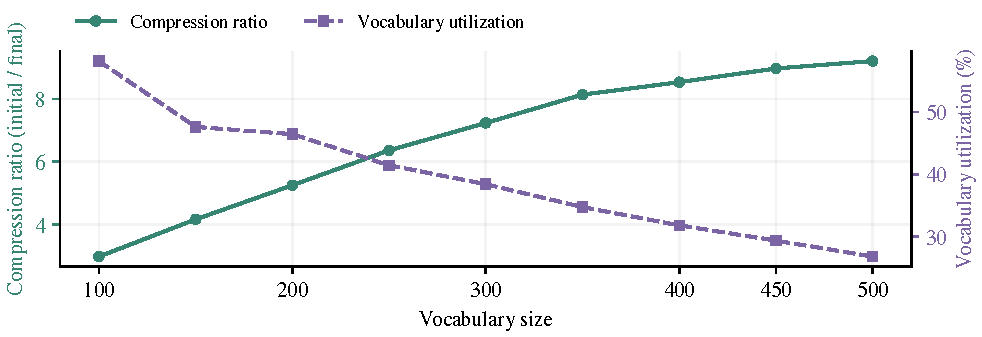
\includegraphics[width=\linewidth]{figures/capacity_tradeoff.pdf}\caption{Compression ratio and vocabulary utilization at different vocabulary sizes on the validation set.}\label{fig:capacity_tradeoff}\end{figure}

We also evaluate tokenizer generalization. We train the tokenizers on relatively simple formulas and test them on complex formulas. The generalization experiment is presented in Appendix~\ref{app:generalization}.


\FloatBarrier
\subsection{Downstream Tasks}
We evaluate the effect of tokenization on PDE discovery. We make two changes to EqGPT (Section~\ref{subsec:changes}), pretrain EqGPT and the modified model (AST-BPE EqGPT) on the small and large corpora, and test whether the models can discover the target PDE from data in the eight cases (Table~\ref{tab:main}).

AST-BPE EqGPT performs better overall on both corpora. With the small corpus, vocabulary sizes of 300 and 450 recover 6 and 7 correct structures, respectively, compared with 3 for EqGPT. With the large corpus, the counts are 3 and 2, compared with 2 for EqGPT. All three models recover fewer cases with the large corpus than with the small corpus. We examine this finding in Section~4.

\begin{table}[H]
\caption[Discovery results for eight cases]{Discovery results for eight cases\protect\footnotemark. Each cell reports Top1 correctness followed by whether Top10 contains the correct structure. \ding{51} denotes success and \ding{55} failure. CD: convection--diffusion; KG: Klein--Gordon; E6: Eq.\ 6.2.12; PD: PDE-divide; CI: Chaffee--Infante. Totals give the number of successful cases for each metric; group maxima are bold.}\label{tab:main}
\centering\fontsize{8.5}{10}\selectfont\setlength{\tabcolsep}{2pt}\begin{tabular*}{\linewidth}{@{\extracolsep{\fill}}llccccccccr@{}}
\toprule
Corpus & Model & Wave & CD & KG & Burgers & E6 & PD & KdV & CI & Total\\
\midrule
212 & EqGPT & \ding{51}/\ding{51} & \ding{55}/\ding{51} & \ding{55}/\ding{51} & \ding{55}/\ding{51} & \ding{55}/\ding{55} & \ding{55}/\ding{51} & \ding{51}/\ding{51} & \ding{51}/\ding{51} & 3/\textbf{7}\\
 & AST-BPE 300 & \ding{51}/\ding{51} & \ding{51}/\ding{51} & \ding{51}/\ding{51} & \ding{51}/\ding{51} & \ding{55}/\ding{55} & \ding{51}/\ding{51} & \ding{51}/\ding{51} & \ding{55}/\ding{51} & 6/\textbf{7}\\
 & AST-BPE 450 & \ding{51}/\ding{51} & \ding{51}/\ding{51} & \ding{51}/\ding{51} & \ding{51}/\ding{51} & \ding{55}/\ding{55} & \ding{51}/\ding{51} & \ding{51}/\ding{51} & \ding{51}/\ding{51} & \textbf{7}/\textbf{7}\\
\midrule
636 & EqGPT & \ding{51}/\ding{51} & \ding{55}/\ding{55} & \ding{55}/\ding{51} & \ding{55}/\ding{51} & \ding{55}/\ding{55} & \ding{55}/\ding{55} & \ding{51}/\ding{51} & \ding{55}/\ding{55} & 2/4\\
 & AST-BPE 300 & \ding{51}/\ding{51} & \ding{55}/\ding{51} & \ding{55}/\ding{51} & \ding{55}/\ding{51} & \ding{55}/\ding{51} & \ding{55}/\ding{55} & \ding{51}/\ding{51} & \ding{51}/\ding{51} & \textbf{3}/\textbf{7}\\
 & AST-BPE 450 & \ding{51}/\ding{51} & \ding{55}/\ding{51} & \ding{55}/\ding{51} & \ding{55}/\ding{51} & \ding{55}/\ding{55} & \ding{55}/\ding{55} & \ding{51}/\ding{51} & \ding{55}/\ding{51} & 2/6\\
\bottomrule
\end{tabular*}
\end{table}
\footnotetext{In the experiments in Table~\ref{tab:main}, both AST-BPE and EqGPT use 20\% random generation.}




\begingroup
\setlength{\intextsep}{2pt}
\setlength{\textfloatsep}{5pt}
\setlength{\floatsep}{4pt}
\setlength{\abovedisplayskip}{5pt}
\setlength{\belowdisplayskip}{5pt}
\setlength{\abovedisplayshortskip}{3pt}
\setlength{\belowdisplayshortskip}{3pt}
\section{Discussion}
\subsection{Corpus Expansion and Candidate Structures}
We analyze all candidate equations generated by the AST-BPE EqGPT models with the two vocabulary sizes in the downstream experiments.\footnote{Candidate statistics in this section are pooled across the eight test cases.} For each vocabulary size and case, we use the structures generated by the small-corpus model as the reference set. A structure generated by the large-corpus model but absent from this set is called a new structure. After corpus expansion, approximately 70--80\% of all candidates have new structures (Table~\ref{tab:changes}).
\begin{table}[H]
\caption{New structures generated by the large-corpus models.}\label{tab:changes}
\centering\small\begin{tabular*}{\linewidth}{@{\extracolsep{\fill}}lrrrr@{}}\toprule
Vocabulary size & Total candidates & New structures & Share(\%) & New structures in Top10\\\midrule
300 & 16,000 & 11,517 & 71.98 & 45/80\\
450 & 16,000 & 12,561 & 78.51 & 48/80\\
\bottomrule\end{tabular*}
\end{table}

\subsection{Analysis of the Reward}
In Eq.~\eqref{eq:reward}, $M$ is the number of terms in the candidate equation, and $R^2=1-\sum_i(y_i-\hat y_i)^2/\sum_i(y_i-\bar y)^2$, where $y_i$ is the value of the fitted left-hand side, $\hat y_i$ is its prediction obtained by least-squares fitting of the remaining terms, and $\bar y$ is the mean of $y_i$.

The reward favors both a good fit to the data and fewer terms. When two structures both describe the current numerical relation well, the one with fewer terms may receive a higher score. We illustrate this with a specific example.

\paragraph{Chaffee--Infante example.}
In the experiment with 636 equations, a vocabulary size of 300, and no random generation, the scoring procedure fits the following new structure:
\begin{equation}\label{eq:wrong}
 \sin(x)u_{xx}+0.002141u_{tt}-0.911730u_{xx}=0.
\end{equation}
The fitted correct structure from the same run is
\begin{equation}\label{eq:correct}
 u^3-1.008575u-0.998787u_t+0.999261u_{xx}=0.
\end{equation}

\begin{table}[H]
\caption{Reward calculation for two candidates. The correct structure has a higher $R^2$ but a stronger four-term penalty.}\label{tab:reward}
\centering\small
\begin{tabular*}{\linewidth}{@{\extracolsep{\fill}}lrrrr@{}}\toprule
Candidate & $M$ & $R^2$ & $1-0.2\log_{10}M$ & Reward\\\midrule
New structure & 3 & 0.991153 & \textbf{0.904576} & \textbf{0.896573}\\
Correct structure & 4 & \textbf{0.999207} & 0.879588 & 0.878891\\\bottomrule
\end{tabular*}
\end{table}

Table~\ref{tab:reward} shows that the correct structure fits the data better, but the new equation has only three terms and receives a higher final score. This shows that the term-count penalty directly reverses the ranking.


Such candidates also occur in other cases. We count special candidate equations generated by the large-corpus models that satisfy all three conditions: \textbf{a new structure, an incorrect structure, and a score above the highest score of any correct structure in the same run}. The results are shown in Table~\ref{tab:special}.
\begin{table}[H]
\caption{Special candidate statistics.}\label{tab:special}
\centering\small\begin{tabular*}{\linewidth}{@{\extracolsep{\fill}}lrrr@{}}\toprule
Vocabulary size & Total candidates & Special candidates & Cases entering Top10\\\midrule
300 & 16,000 & 7 & 4/8\\
450 & 16,000 & 18 & 4/8\\
\bottomrule\end{tabular*}
\end{table}

\begin{samepage}
We therefore consider the following explanation for the decline in PDE discovery after corpus expansion: \textbf{The larger corpus leads the model to generate more diverse equation structures. A small number of new equations fit the data nearly as well as the target equation but contain fewer terms, and therefore receive higher rewards. Although there are few such equations, they enter Top10 in four cases at each vocabulary size. Candidates with the target structure are then ranked lower and are less likely to be selected, reducing the ability to discover the target PDE from data.}


\section{Conclusion}
\begin{itemize}\setlength{\itemsep}{0pt}\setlength{\parsep}{0pt}
\item AST-BPE performs better than general-purpose tokenizers on the upstream tasks.
\item AST-BPE can substantially improve the PDE discovery ability of EqGPT.
\item Training on the larger corpus instead reduces PDE discovery performance.
\end{itemize}

The code, results, and other materials for this paper are available in the following GitHub repository:\\
\url{https://github.com/xtr1976536/from-tokenizer-to-pde-discovery-1}

\end{samepage}
\endgroup
\FloatBarrier
\clearpage
\appendix
\section{Full Experimental Parameters and Processing}\label{app:params}
Table~\ref{tab:params} lists the model, training, and search parameters.
\begin{table}[H]
\caption{Model, pretraining, and search parameters.}\label{tab:params}
\centering\small
\renewcommand{\arraystretch}{1.22}
\begin{tabular*}{\linewidth}{@{\extracolsep{\fill}}p{3.05in}p{3.25in}@{}}\toprule
Parameter & Value\\\midrule
Transformer layers / attention heads & 6 / 8\\
Model dimension / feed-forward dimension & 768 / 2048\\
Key and value dimensions per head & 64 / 64\\
Position capacity / maximum generation length & 72 / 70\\\midrule
Pretraining optimizer / batch size & Adam / 128\\
Initial / minimum learning rate & $10^{-4}$ / $10^{-6}$\\
Cosine period / training limit & 200 / 200 epochs\\
Validation metric / evaluation frequency & Validation cross-entropy / every epoch\\
Early-stopping patience / minimum improvement & 15 epochs / $10^{-5}$\\
Gradient clipping norm & 1\\
Commutative variants per formula & 32\\\midrule
Search rounds / scored candidates per round & 5 / 400\\
Maximum attempts per round & 5,000\\
SFT training samples & Up to 10 sequences in the cumulative Top10\\
SFT epochs per round & 5 epochs\\
SFT initial / minimum learning rate & $10^{-5}$ / $10^{-7}$\\
SFT learning-rate schedule & Cosine decay, restarted each round\\
Numerical-cache seed & 525\\
Model initialization and search seeds & 525, 526, 527\\\bottomrule
\end{tabular*}
\end{table}


\section{Discovery Results by Seed}\label{app:seeds}
Table~\ref{tab:seeds} lists the results for seeds 526 and 527 in each case. Cells have the same meaning as in Table~\ref{tab:main}; model sampling uses no uniform random distribution, while random sampling uses the 20\% mixture.
\begingroup
\fontsize{9}{11}\selectfont
\setlength{\tabcolsep}{2pt}
\renewcommand{\arraystretch}{1.15}
\captionof{table}{Structure discovery results for the other random seeds.}\label{tab:seeds}
\setlength{\LTleft}{0pt}\setlength{\LTright}{0pt}
\begin{longtable}{@{}p{.45in}p{.45in}p{1.12in}*{8}{>{\centering\arraybackslash}p{.39in}}>{\centering\arraybackslash}p{.47in}@{}}
\toprule Corpus & Seed & Setting & Wave & CD & KG & Burgers & E6 & PD & KdV & CI & Total\\\midrule
\endfirsthead
\toprule Corpus & Seed & Setting & Wave & CD & KG & Burgers & E6 & PD & KdV & CI & Total\\\midrule
\endhead
\bottomrule\endfoot
212 & 526 & EqGPT & \ding{51}/\ding{51} & \ding{55}/\ding{51} & \ding{55}/\ding{51} & \ding{55}/\ding{51} & \ding{55}/\ding{55} & \ding{51}/\ding{51} & \ding{51}/\ding{51} & \ding{55}/\ding{51} & 3/\textbf{7}\\
212 & 526 & 200 model & \ding{51}/\ding{51} & \ding{51}/\ding{51} & \ding{51}/\ding{51} & \ding{51}/\ding{51} & \ding{55}/\ding{55} & \ding{55}/\ding{51} & \ding{51}/\ding{51} & \ding{55}/\ding{51} & 5/\textbf{7}\\
212 & 526 & 200 random & \ding{51}/\ding{51} & \ding{51}/\ding{51} & \ding{51}/\ding{51} & \ding{51}/\ding{51} & \ding{55}/\ding{55} & \ding{51}/\ding{51} & \ding{51}/\ding{51} & \ding{51}/\ding{51} & \textbf{7}/\textbf{7}\\
212 & 526 & 300 model & \ding{51}/\ding{51} & \ding{51}/\ding{51} & \ding{51}/\ding{51} & \ding{51}/\ding{51} & \ding{55}/\ding{55} & \ding{55}/\ding{51} & \ding{51}/\ding{51} & \ding{51}/\ding{51} & 6/\textbf{7}\\
212 & 526 & 300 random & \ding{51}/\ding{51} & \ding{55}/\ding{51} & \ding{55}/\ding{51} & \ding{51}/\ding{51} & \ding{55}/\ding{55} & \ding{55}/\ding{51} & \ding{51}/\ding{51} & \ding{51}/\ding{51} & 4/\textbf{7}\\
212 & 526 & 450 model & \ding{51}/\ding{51} & \ding{51}/\ding{51} & \ding{51}/\ding{51} & \ding{51}/\ding{51} & \ding{55}/\ding{55} & \ding{55}/\ding{51} & \ding{51}/\ding{51} & \ding{51}/\ding{51} & 6/\textbf{7}\\
212 & 526 & 450 random & \ding{51}/\ding{51} & \ding{51}/\ding{51} & \ding{51}/\ding{51} & \ding{51}/\ding{51} & \ding{55}/\ding{55} & \ding{55}/\ding{55} & \ding{51}/\ding{51} & \ding{51}/\ding{51} & 6/6\\
\midrule
212 & 527 & EqGPT & \ding{51}/\ding{51} & \ding{55}/\ding{51} & \ding{55}/\ding{51} & \ding{55}/\ding{51} & \ding{55}/\ding{55} & \ding{55}/\ding{51} & \ding{51}/\ding{51} & \ding{55}/\ding{51} & 2/7\\
212 & 527 & 200 model & \ding{51}/\ding{51} & \ding{51}/\ding{51} & \ding{51}/\ding{51} & \ding{51}/\ding{51} & \ding{55}/\ding{55} & \ding{51}/\ding{51} & \ding{51}/\ding{51} & \ding{51}/\ding{51} & \textbf{7}/7\\
212 & 527 & 200 random & \ding{51}/\ding{51} & \ding{51}/\ding{51} & \ding{51}/\ding{51} & \ding{51}/\ding{51} & \ding{55}/\ding{55} & \ding{51}/\ding{51} & \ding{51}/\ding{51} & \ding{51}/\ding{51} & \textbf{7}/7\\
212 & 527 & 300 model & \ding{51}/\ding{51} & \ding{51}/\ding{51} & \ding{51}/\ding{51} & \ding{51}/\ding{51} & \ding{55}/\ding{55} & \ding{55}/\ding{51} & \ding{51}/\ding{51} & \ding{55}/\ding{51} & 5/7\\
212 & 527 & 300 random & \ding{51}/\ding{51} & \ding{51}/\ding{51} & \ding{51}/\ding{51} & \ding{51}/\ding{51} & \ding{51}/\ding{51} & \ding{55}/\ding{51} & \ding{51}/\ding{51} & \ding{51}/\ding{51} & \textbf{7}/\textbf{8}\\
212 & 527 & 450 model & \ding{51}/\ding{51} & \ding{51}/\ding{51} & \ding{51}/\ding{51} & \ding{51}/\ding{51} & \ding{55}/\ding{55} & \ding{55}/\ding{51} & \ding{51}/\ding{51} & \ding{55}/\ding{51} & 5/7\\
212 & 527 & 450 random & \ding{51}/\ding{51} & \ding{51}/\ding{51} & \ding{51}/\ding{51} & \ding{51}/\ding{51} & \ding{55}/\ding{55} & \ding{55}/\ding{51} & \ding{51}/\ding{51} & \ding{55}/\ding{51} & 5/7\\
\midrule
636 & 526 & EqGPT & \ding{51}/\ding{51} & \ding{55}/\ding{55} & \ding{55}/\ding{55} & \ding{55}/\ding{55} & \ding{55}/\ding{55} & \ding{55}/\ding{55} & \ding{51}/\ding{51} & \ding{55}/\ding{51} & 2/3\\
636 & 526 & 200 model & \ding{51}/\ding{51} & \ding{55}/\ding{51} & \ding{55}/\ding{51} & \ding{55}/\ding{55} & \ding{55}/\ding{55} & \ding{55}/\ding{51} & \ding{51}/\ding{51} & \ding{55}/\ding{51} & 2/6\\
636 & 526 & 200 random & \ding{51}/\ding{51} & \ding{55}/\ding{51} & \ding{51}/\ding{51} & \ding{55}/\ding{51} & \ding{55}/\ding{55} & \ding{55}/\ding{51} & \ding{51}/\ding{51} & \ding{55}/\ding{51} & 3/\textbf{7}\\
636 & 526 & 300 model & \ding{51}/\ding{51} & \ding{55}/\ding{51} & \ding{51}/\ding{51} & \ding{55}/\ding{51} & \ding{55}/\ding{55} & \ding{55}/\ding{51} & \ding{51}/\ding{51} & \ding{55}/\ding{51} & 3/\textbf{7}\\
636 & 526 & 300 random & \ding{51}/\ding{51} & \ding{55}/\ding{51} & \ding{51}/\ding{51} & \ding{55}/\ding{51} & \ding{51}/\ding{51} & \ding{55}/\ding{55} & \ding{51}/\ding{51} & \ding{55}/\ding{51} & \textbf{4}/\textbf{7}\\
636 & 526 & 450 model & \ding{51}/\ding{51} & \ding{55}/\ding{51} & \ding{55}/\ding{55} & \ding{55}/\ding{51} & \ding{55}/\ding{55} & \ding{55}/\ding{51} & \ding{51}/\ding{51} & \ding{55}/\ding{51} & 2/6\\
636 & 526 & 450 random & \ding{51}/\ding{51} & \ding{55}/\ding{51} & \ding{51}/\ding{51} & \ding{55}/\ding{51} & \ding{55}/\ding{55} & \ding{55}/\ding{51} & \ding{51}/\ding{51} & \ding{55}/\ding{51} & 3/\textbf{7}\\
\midrule
636 & 527 & EqGPT & \ding{51}/\ding{51} & \ding{55}/\ding{51} & \ding{55}/\ding{51} & \ding{55}/\ding{51} & \ding{55}/\ding{55} & \ding{55}/\ding{55} & \ding{51}/\ding{51} & \ding{55}/\ding{55} & 2/5\\
636 & 527 & 200 model & \ding{51}/\ding{51} & \ding{55}/\ding{51} & \ding{51}/\ding{51} & \ding{55}/\ding{55} & \ding{55}/\ding{55} & \ding{55}/\ding{51} & \ding{51}/\ding{51} & \ding{55}/\ding{51} & 3/6\\
636 & 527 & 200 random & \ding{51}/\ding{51} & \ding{51}/\ding{51} & \ding{51}/\ding{51} & \ding{51}/\ding{51} & \ding{55}/\ding{55} & \ding{55}/\ding{55} & \ding{51}/\ding{51} & \ding{55}/\ding{51} & \textbf{5}/6\\
636 & 527 & 300 model & \ding{51}/\ding{51} & \ding{55}/\ding{51} & \ding{55}/\ding{51} & \ding{55}/\ding{51} & \ding{55}/\ding{55} & \ding{55}/\ding{51} & \ding{51}/\ding{51} & \ding{55}/\ding{51} & 2/7\\
636 & 527 & 300 random & \ding{51}/\ding{51} & \ding{55}/\ding{51} & \ding{55}/\ding{51} & \ding{55}/\ding{51} & \ding{51}/\ding{51} & \ding{51}/\ding{51} & \ding{51}/\ding{51} & \ding{55}/\ding{51} & 4/\textbf{8}\\
636 & 527 & 450 model & \ding{51}/\ding{51} & \ding{51}/\ding{51} & \ding{51}/\ding{51} & \ding{55}/\ding{51} & \ding{55}/\ding{55} & \ding{55}/\ding{51} & \ding{51}/\ding{51} & \ding{55}/\ding{51} & 4/7\\
636 & 527 & 450 random & \ding{55}/\ding{55} & \ding{55}/\ding{51} & \ding{51}/\ding{51} & \ding{55}/\ding{51} & \ding{55}/\ding{55} & \ding{55}/\ding{51} & \ding{51}/\ding{51} & \ding{55}/\ding{51} & 2/6\\

\end{longtable}\addtocounter{table}{-1}
\endgroup
\normalsize

\section{Effect of Random Sampling on Discovery}\label{app:sampling}
Figure~\ref{fig:vocab_sampling} compares vocabulary sizes and sampling settings for seed 525. With 212 equations, random generation raises Top1 from 4/8 to 7/8 at vocabulary size 200, from 5/8 to 6/8 at size 300, and from 5/8 to 7/8 at size 450. All three settings benefit from mixed sampling for seed 525.

Random sampling has a slightly different effect with the large corpus (Top1 decreases at vocabulary size 300).

\begin{figure}[H]\centering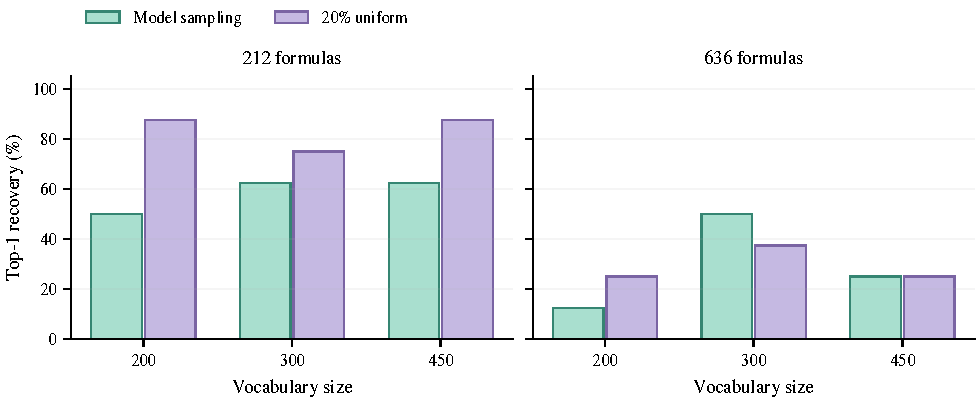
\includegraphics[width=\linewidth]{figures/vocab_sampling.pdf}\caption{Vocabulary-size and random-generation comparison for seed 525. Model sampling uses no random mixture; 20\% uniform adds uniform random tokens.}\label{fig:vocab_sampling}\end{figure}






\FloatBarrier
\section{Simple-to-Complex Generalization}\label{app:generalization}
Formula complexity is
\begin{equation*}
 K=0.40h(L/60)+0.20h(C_{\rm cmd}/6)+0.15h(D/3)+0.15h(S/18)+0.10h(O/12),\quad h(v)=\min(v,2),
\end{equation*}
The five components are computed from the LaTeX source. Consider \verb|(\Delta{u})=0|:
\begin{itemize}\setlength{\itemsep}{3pt}\setlength{\parsep}{0pt}
\item \textbf{Number of lexical units $L$.} Split the source into complete LaTeX commands, complete numeric strings, and other individual characters, ignoring whitespace. Count repeated occurrences separately. Here the units are \verb|(|, \verb|\Delta|, \verb|{|, \verb|u|, \verb|}|, \verb|)|, \verb|=|, and \verb|0|, so $L=8$.
\item \textbf{Number of LaTeX command types $C_{\rm cmd}$.} Count distinct commands consisting of a backslash followed by English letters. Repeated occurrences of a command count as one type. The only command here is \verb|\Delta|, so $C_{\rm cmd}=1$.
\item \textbf{Maximum bracket nesting depth $D$.} Each opening parenthesis, brace, or square bracket increases the depth by one; a closing bracket decreases it by one. Take the largest depth. Here \verb|{u}| is nested within \verb|(...)|, so $D=2$.
\item \textbf{Number of non-bracket symbol types $S$.} Remove the six bracket characters and count distinct lexical units, treating each command and numeric string as a unit. The remaining units here are \verb|\Delta|, \verb|u|, \verb|=|, and \verb|0|, so $S=4$.
\item \textbf{Number of operators $O$.} Count occurrences of \verb|+ - * / = < > ^ _| and \verb|\sum|, \verb|\prod|, \verb|\int|, \verb|\partial|, \verb|\nabla|, \verb|\frac|, and \verb|\sqrt|. Here only \verb|=| is counted; \verb|\Delta| is not in this set, so $O=1$.
\end{itemize}
Substituting $(L,C_{\rm cmd},D,S,O)=(8,1,2,4,1)$ gives $K=0.2283$.

After sorting by complexity, the lowest 30\% are simple formulas (191), the highest 30\% are complex formulas (190), and the remaining 255 are moderate. The experiment trains on the 173 simple formulas in the training split and evaluates on the 27 and 21 complex formulas in the validation and test splits. AST-BPE achieves test compression ratios of 5.426 and 6.138, above the 1.758--1.834 of the general-purpose tokenizers, while preserving complete commands.
\begin{table}[H]
\caption{Training on simple formulas and testing on complex formulas; 21 test formulas. Metrics are the same as in Table~\ref{tab:upstream}.}\label{tab:generalization}
\centering\small\begin{tabular*}{\linewidth}{@{\extracolsep{\fill}}lrrrr@{}}\toprule
Tokenizer & Compression ratio$\uparrow$ & Command integrity(\%) & Number integrity(\%) & Utilization(\%)\\\midrule
AST-BPE 300 & 5.426 & \textbf{100.0} & 100.0 & 21.6\\
AST-BPE 450 & \textbf{6.138} & \textbf{100.0} & 100.0 & 16.0\\
Qwen2.5 & 1.834 & 0.0 & 100.0 & --\\
Llama 3 & 1.834 & 0.0 & 100.0 & --\\
\texttt{o200k\_base} & 1.758 & 0.0 & 100.0 & --\\
\bottomrule\end{tabular*}
\end{table}


\clearpage
\section{Token Frequency Distributions across Corpora and Vocabulary Sizes}\label{app:token_frequency}
\begin{figure}[H]
\centering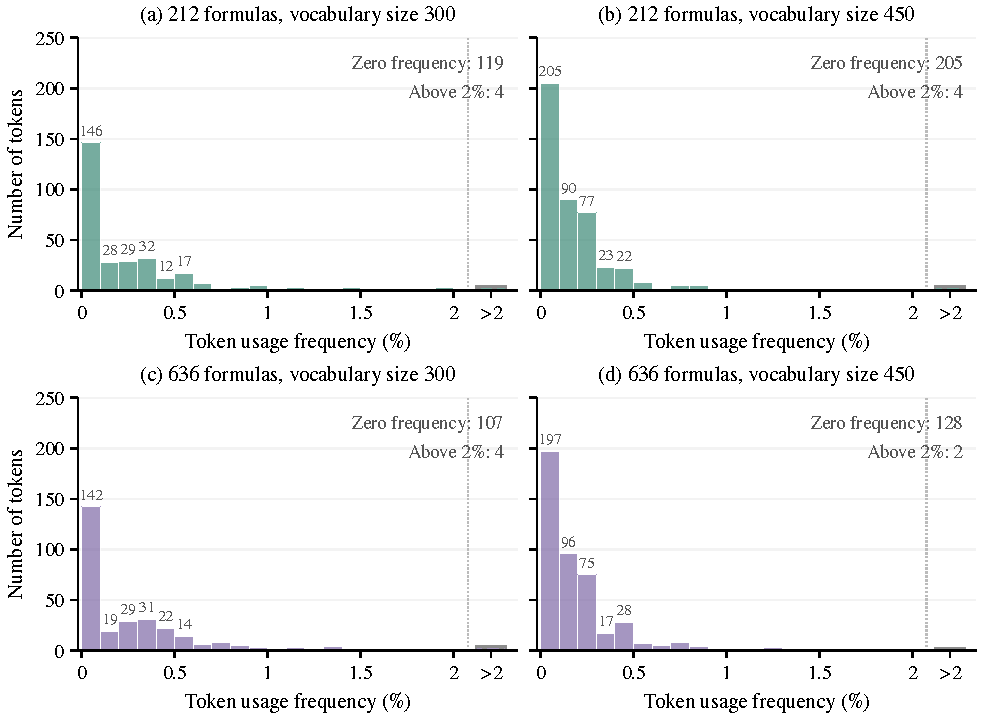
\includegraphics[width=\linewidth]{figures/token_id_frequency.pdf}
\caption{Histogram of token usage frequencies. The horizontal axis gives each token's share of all token occurrences, and the vertical axis gives the number of tokens in each interval. The bar width is 0.1 percentage points; zero-frequency tokens are included in the first bar.}\label{fig:token_frequency}
\end{figure}

Tokens in all four vocabularies are concentrated in the low-frequency intervals. Only a few tokens have frequencies above 2\%, giving right-skewed distributions. There are 119 and 205 zero-frequency tokens in the small-corpus vocabularies and 107 and 128 in the large-corpus vocabularies.

At each vocabulary size, the large corpus uses more distinct tokens: the counts increase from 178 and 242 to 190 and 319. When vocabulary size increases from 300 to 450, the zero-frequency share rises from 40.1\% to 45.9\% for the small corpus, but falls from 36.0\% to 28.6\% for the large corpus.

\end{document}
